\documentclass[11pt,a4paper]{article}
\usepackage{graphicx,psfig,fancyhdr,natbib,subfigure}
\usepackage{epsfig, psfig, epsf}
\usepackage{amsmath, cancel}
\usepackage{amssymb}
%\usepackage{lscape}
\usepackage{dcolumn}% Align table columns on decimal point
\usepackage{bm}% bold math
\usepackage{hyperref,ifthen}
\usepackage{verbatim}



%%%%%%%%%%%%%%%%%%%%%%%%%%%%%%%%%%%%%%%%%%%
%       define Journal abbreviations      %
%%%%%%%%%%%%%%%%%%%%%%%%%%%%%%%%%%%%%%%%%%%
\def\nat{Nat} \def\apjl{ApJ~Lett.} \def\apj{ApJ}
\def\apjs{ApJS} \def\aj{AJ} \def\mnras{MNRAS}
\def\prd{Phys.~Rev.~D} \def\prl{Phys.~Rev.~Lett.}
\def\plb{Phys.~Lett.~B} \def\jhep{JHEP}
\def\npbps{NUC.~Phys.~B~Proc.~Suppl.} \def\prep{Phys.~Rep.}
\def\pasp{PASP} \def\aap{Astron.~\&~Astrophys.} \def\araa{ARA\&A}
\def\jcap{\ref@jnl{J. Cosmology Astropart. Phys.}} 
\def\nar{New~A.R.} 

\newcommand{\preep}[1]{{\tt #1} }

%%%%%%%%%%%%%%%%%%%%%%%%%%%%%%%%%%%%%%%%%%%%%%%%%%%%%
%              define symbols                       %
%%%%%%%%%%%%%%%%%%%%%%%%%%%%%%%%%%%%%%%%%%%%%%%%%%%%%
\def \Mpc {~{\rm Mpc} }
\def \Om {\Omega_0}
\def \Omb {\Omega_{\rm b}}
\def \Omcdm {\Omega_{\rm CDM}}
\def \Omlam {\Omega_{\Lambda}}
\def \Omm {\Omega_{\rm m}}
\def \ho {H_0}
\def \qo {q_0}
\def \lo {\lambda_0}
\def \kms {{\rm ~km~s}^{-1}}
\def \kmsmpc {{\rm ~km~s}^{-1}~{\rm Mpc}^{-1}}
\def \hmpc{~\;h^{-1}~{\rm Mpc}} 
\def \hkpc{\;h^{-1}{\rm kpc}} 
\def \hmpcb{h^{-1}{\rm Mpc}}
\def \dif {{\rm d}}
\def \mlim {m_{\rm l}}
\def \bj {b_{\rm J}}
\def \mb {M_{\rm b_{\rm J}}}
\def \mg {M_{\rm g}}
\def \mi {M_{\rm i}}
\def \qso {_{\rm QSO}}
\def \lrg {_{\rm LRG}}
\def \gal {_{\rm gal}}
\def \xibar {\bar{\xi}}
\def \xis{\xi(s)}
\def \xisp{\xi(\sigma, \pi)}
\def \Xisig{\Xi(\sigma)}
\def \xir{\xi(r)}
\def \max {_{\rm max}}
\def \gsim { \lower .75ex \hbox{$\sim$} \llap{\raise .27ex \hbox{$>$}} }
\def \lsim { \lower .75ex \hbox{$\sim$} \llap{\raise .27ex \hbox{$<$}} }
\def \deg {^{\circ}}
%\def \sqdeg {\rm deg^{-2}}
\def \deltac {\delta_{\rm c}}
\def \mmin {M_{\rm min}}
\def \mbh  {M_{\rm BH}}
\def \mdh  {M_{\rm DH}}
\def \msun {M_{\odot}}
\def \z {_{\rm z}}
\def \edd {_{\rm Edd}}
\def \lin {_{\rm lin}}
\def \nonlin {_{\rm non-lin}}
\def \wrms {\langle w_{\rm z}^2\rangle^{1/2}}
\def \dc {\delta_{\rm c}}
\def \wp {w_{p}(\sigma)}
\def \PwrSp {\mathcal{P}(k)}
\def \DelSq {$\Delta^{2}(k)$}
\def \WMAP {{\it WMAP \,}}
\def \cobe {{\it COBE }}
\def \COBE {{\it COBE \;}}
\def \HST  {{\it HST \,\,}}
\def \Spitzer  {{\it Spitzer \,}}
\def \ATLAS {VST-AA$\Omega$ {\it ATLAS} }
\def \BEST   {{\tt best} }
\def \TARGET {{\tt target} }
\def \TQSO   {{\tt TARGET\_QSO}}
\def \HIZ    {{\tt TARGET\_HIZ}}
\def \FIRST  {{\tt TARGET\_FIRST}}
\def \zc {z_{\rm c}}
\def \zcz {z_{\rm c,0}}


\newcommand{\sqdeg}{deg$^{-2}$}
\newcommand{\lya}{Ly$\alpha$\ }
%\newcommand{\lya}{Ly\,$\alpha$\ }
\newcommand{\lyaf}{Ly\,$\alpha$\ forest}
%\newcommand{\eg}{e.g.~}
%\newcommand{\etal}{et~al.~}
\newcommand{\cii}{C\,{\sc ii}\ }
\newcommand{\ciii}{C\,{\sc iii}]\ }
\newcommand{\civ}{C\,{\sc iv}\ }
\newcommand{\SiIV}{Si\,{\sc iv}\ }
\newcommand{\mgii}{Mg\,{\sc ii}\ }
\newcommand{\feii}{Fe\,{\sc ii}\ }
\newcommand{\feiii}{Fe\,{\sc iii}\ }
\newcommand{\caii}{Ca\,{\sc ii}\ }
\newcommand{\halpha}{H\,$\alpha$\ }
\newcommand{\hbeta}{H\,$\beta$\ }
\newcommand{\oi}{[O\,{\sc i}]\ }
\newcommand{\oii}{[O\,{\sc ii}]\ }
\newcommand{\oiii}{[O\,{\sc iii}]\ }
\newcommand{\heii}{[He\,{\sc ii}]\ }
\newcommand{\nii}{N\,{\sc ii}\ }
\newcommand{\nv}{N\,{\sc v}\ }

%% From:: /cos_pc19a_npr/LaTeX/proposals/JWST/JWST_ERS/Proposal/lines.tex
%%  
\newcommand{\imw}{$i$--$W3$}
\newcommand{\imwf}{$i$--$W4$}
\newcommand{\rmwf}{$r$--$W4$}
\newcommand{\imwt}{$i$--$W2$}
\newcommand{\wtmwf}{$W3$--$W4$}
%\newcommand{\kms}{km s$^{-1}$}
\newcommand{\cmN}{cm$^{-2}$}
\newcommand{\cmn}{cm$^{-3}$}
%\newcommand{\msun}{M$_{\odot}$}
\newcommand{\lsun}{L$_{\odot}$}
\newcommand{\lam}{$\lambda$}
\newcommand{\mum}{$\mu$m}
\newcommand{\ebv}{$E(B$$-$$V)$}
%\newcommand{\heii}{\mbox{He\,{\sc ii}}}
\newcommand{\cv}{\mbox{C\,{\sc v}}}
%\newcommand{\civ}{\mbox{C\,{\sc iv}}}
%\newcommand{\ciii}{\mbox{C\,{\sc iii}}}
%\newcommand{\cii}{\mbox{C\,{\sc ii}}}
%\newcommand{\nv}{\mbox{N\,{\sc v}}}
\newcommand{\niv}{\mbox{N\,{\sc iv}}}
\newcommand{\niii}{\mbox{N\,{\sc iii}}}
%\newcommand{\oi}{\mbox{O\,{\sc i}}}
%\newcommand{\oii}{\mbox{O\,{\sc ii}}}
%\newcommand{\oiii}{\mbox{[O\,{\sc iii}]}}
\newcommand{\oiv}{\mbox{O\,{\sc iv}}}
\newcommand{\ov}{\mbox{O\,{\sc v}}}
\newcommand{\ovi}{\mbox{O\,{\sc vi}}}
\newcommand{\ovii}{\mbox{O\,{\sc vii}}}

%\newcommand{\feii}{\mbox{Fe\,{\sc ii}}}
%\newcommand{\feiii}{\mbox{Fe\,{\sc iii}}}
%\newcommand{\mgii}{\mbox{Mg\,{\sc ii}}}
\newcommand{\neii}{[Ne\,{\sc ii}]\ }
\newcommand{\neiii}{[Ne\,{\sc ii}]\ }
\newcommand{\nev}{Ne\,{\sc v}\ }
\newcommand{\nevi}{[Ne\,{\sc vi}]\ }
\newcommand{\neviii}{\mbox{Ne\,{\sc viii}}}
\newcommand{\aliii}{\mbox{Al\,{\sc iii}}}
\newcommand{\siii}{\mbox{Si\,{\sc ii}}}
\newcommand{\siiii}{\mbox{Si\,{\sc iii}}}
\newcommand{\siiv}{\mbox{Si\,{\sc iv}}}
%\newcommand{\lya}{\mbox{Ly$\alpha$}}
%\newcommand{\lyb}{\mbox{Ly$\beta$}}
\newcommand{\hi}{\mbox{H\,{\sc i}}}
\newcommand{\snine}{\mbox{[S\,{\sc ix}]}}
\newcommand{\sivi}{\mbox{[Si\,{\sc vi}]}}
\newcommand{\sivii}{\mbox[{Si\,{\sc vii}]}}
\newcommand{\siix}{\mbox{[Si\,{\sc ix}]}}
\newcommand{\six}{\mbox{[Si\,{\sc x}]}}
\newcommand{\sixi}{\mbox{[Si\,{\sc xi}]}}
\newcommand{\caviii}{\mbox{[Ca\,{\sc viii}]}}
\newcommand{\arii}{\mbox{[Ar\,{\sc ii}]}}

%%[Ar II] 6.97
%% [S IX] 1.252 μm 328 
% [Si X] 1.430 μm 351 
% [Si XI] 1.932 μm 401 
% [Si VI] 1.962 μm 167 
% [Ca VIII] 2.321 μm 128 
% [Si VII] 2.483 μm 205 
% [Si IX] 3.935 μm 303
% [Ar II] 6.97


%\snine\ at 1.252$\mu$m, \six\ at 1.430$\mu$m, \sixi\ at 1.932$\mu$m, \sivi\ at
%1.962$\mu$m, \caviii\ at 2.321$\mu$m, \sivi\ at 2.483$\mu$m \siix\ at
%3.935$\mu$m and \arii\ at 6.97$\mu$m. 
%%
%% such as [Ne ii]12.8 μm, [Ne v]14.3 μm, [Ne iii]15.5 μm, [S iii]18.7 μm and 33.48 μm, [O iv]25.89 μm and [Si ii]34.8 μm (e.g
%%
%% MIR emission lines like [NeII] and [NeV] are ..
%%
%% Also,  arXiv:astro-ph/0003457v1 
%% [NeV] 14.32um & 24.32um and [NeVI] 7.65um imply an A(V)>160 towards the NLR...
%% [NeIII]15.56um/[NeII]12.81um
%%
%% [Ne V] 14.3, 24.2 μm 97.
%% [Ne II] 12.8 μm
%% [OIV] 26μm
%%


\setlength {\textwidth}{160mm} 
\setlength {\textheight}{255mm}
\topmargin=-15.00mm
\oddsidemargin=-5.0mm

\begin{document}

\title{Supplemental Material}
\maketitle

Further selection and observational details are presented here. We
report the photometric qualities that led to J1100-0053 being targeted
and the specifics of the repeat spectroscopy. We also discuss
alternative scenarios that could explain the observations, and why we
dismiss these in turn, while giving further details of our preferred
model.


\section{Further Observational Details}

\subsection{Optical Imaging}
SDSS J110057.70-005304.5 was first detected in the National Geographic
Society-Palomar Observatory Sky Survey \cite[NGS-POSS; ][]{Abell1959,
Minkowski_Abell1963book} in 1955 April. It is catalogued in the
SuperCOSMOS Science Archive \cite[\href{http://ssa.roe.ac.uk/}{SSA};
][]{Hambly2001_I, Hambly2001_II} and due to its equatorial position
was also observed by the UK Schmidt Telescope \cite[UKST;
][]{Cannon1975, Cannon1979book}. Querying the SSA returns {\it
gCorMag} and {\it sCorMag} which are the magnitudes assuming the
object is either a galaxy or star, respectively. We use the {\it
sCorMag} values as is appropriate for an image with flux dominated by
the point-like AGN; the {\it sCorMag} magnitudes are calibrated in the
Vega system. For J1100-0053 we find the magnitudes are: 18.10 mag in
the blue UK-J filter from MJD 45440.47 (1983 April 16); 17.49 mag in
the red POSS-I 'E'-filter from MJD 35214.22 (1955 April 17); 17.92 mag
in the red UK-R filter from MJD 46521.47 (1986 April 01) and 17.71 mag
in the UK-I filter from MJD 47273.49 (1988 April 22). J1100-0053 is
not in the Digital Access to a Sky Century @ Harvard
(DASCH\footnote{http://dasch.rc.fas.harvard.edu/project.php}).

J1100-0053 was observed by R\"{o}ntgensatellit (ROSAT) and appears in
the All-Sky Survey Bright Source Catalogue \citep[RASS-BSC;
][]{Appenzeller1998, Voges1999}.  J1100-0053 was imaged by the Sloan
Digital Sky Survey (SDSS) in the $u$, $g$, $r$, $i$ and $z$-bands and
satisfied a number of spectroscopic targeting flags making it a quasar
target \citep{Richards2002}.  J1100-0053 is in Data Release 3 (DR3) of
the Dark Energy Camera Legacy Survey (DECaLS), where there are 8, 3
and 9 exposures in the $g$, $r$ and $z$-band respectively. The $g$-
and $r$-band observations span roughly a year, ($56707 \leq g_{\rm
MJD} \leq 56727$ and $56367 \leq r_{\rm MJD} \leq 56367$), while the
$z$-band observations span almost 3 years ($56383 \leq z_{\rm MJD}
\leq 57398)$.

\subsection{SDSS and BOSS Spectroscopy}
A spectrum was obtained on MJD 51908 (SDSS Plate 277, Fiber 212) and
the spectrum of a $z=0.378$ quasar was catalogued in the SDSS Early
Data Release \citep{Stoughton2002, Schneider2002}. The physical
properties of J1100-0053 derived from the MJD 51908 spectrum using the
methods in \citet{Shen2011}, are given in Table~\ref{tab:Shen_props},
where we also give the properties of J2314+0005 \citep{Guo2016} and
J1052+1519 \citep{Stern2018} for comparison.

\begin{table}[]
  \centering
  \begin{tabular}{l l l l}
    \hline \hline 
    &&\\
    Quantity                                          &     this paper                       &  Guo et al. (2016)              & Stern et al. (2018) \\
    &&\\
    \hline 
    &&\\
    SDSS name                                       &    J110057.70-005304.5    &  J231742.60+000535.1    & J105203.55+151929.5 \\
    R.A. / deg                                        &  165.240463                       &  349.42752075                &   163.01480103  \\
    Declination / deg                            &   -0.884586                        &   +0.093091                    & 15.32488632 \\
    redshift, $z$                                    &   0.3778$\pm$0.0003        & 0.3209$\pm$0.0002       & 0.3022$\pm$0.0008\\
    &&\\ 
    
    \multirow{3}{*}{SDSS Plate, Fiber, MJD }  &  	277, 212,   51908(*)    &  382, 173, 51816(*)         & 2483, 204, 53852(*) \\
    &                                           & 679, 551, 52177              & \\    
    &                                           & 680, 346, 52200             & \\
    BOSS Plate, Fiber, MJD                 & 	3836, 258, 55302          	    &    --                                & -- \\
    &&\\ 
    $M_{i}(z=2)$  / mag                          &   -24.48                             & -23.65                           & -22.73 \\
    log $(L_{\rm bol} / {\rm erg s}^{-1}) $  &   45.78$\pm$0.02               & 45.56$\pm$0.004      & 45.07$\pm$0.004 \\
    % log $(L_{\rm Edd} / {\rm erg s}^{-1}) $  &  46.93                        & 46.53                   & 46.56
    log $(M_{\rm BH} / M_{\odot})  $           &  8.83$\pm$0.14                & 8.43$\pm$0.03           & 8.46$\pm$0.02 \\
    Eddington ratio  (\%)                        &        7.0                         &  10.7                           &  3.2     \\ 
    &&\\
    \hline \hline 
  \end{tabular}
  \caption{Physical properties of J1100-0053, J2317+0005 and
    J1052+1519 using the methods from \citet{Shen2011}. (*)This spectrum
    was used to estimate the quantities reported.
    %% $L_{\rm Edd}  =  \frac{4 \pi G M m_{\rm p} c} {\sigma_{T}}  = 1.26\times10^{38}\left (M/M_{\odot}  \right )$ erg s$^{-1}$.
} 
 \label{tab:Shen_props}
\end{table}

The second epoch spectrum is from the SDSS-III Baryon Oscillation
Spectroscopic Survey \citep[BOSS; ][]{Dawson2013} and shows the
downturn at $\lesssim$4300\AA. SDSS-III BOSS actively vetoed known
$z<2$ QSOs \citep{Ross2012}, but due to J1100-0053 being selected as
an ancillary target \citep[via a white dwarf program;][]{Kepler2015,
Kepler2016} a second spectral epoch was obtained. Due to a design
tradeoff to improve throughput in the Ly$\alpha$-forest of quasar
spectra in BOSS, QSO targets were subject to spectrophotometric
calibration errors \citep{Margala2016}. These are introduced primarily
due to offsets in fiber-hole positioning between quasar targets and
spectrophotometric standard stars. However, since J1100-0053 was {\it
not} a BOSS QSO {\it target}, it is not subject to this ``blue
offset''. J1100-0053 has no pipeline flag suggesting the spectrum was
compromised during data taking. We checked the calibration of BOSS
Plate 3836 that observed J1100-0053 and confirmed that the data were
high-SNR and that the behaviour in the blue spectrum was not due to
the instrument, telescope or data reduction.


\subsubsection{Palomar Spectroscopy} 
A third epoch spectrum was obtained from the Palomar Hale 5m telescope
using the Double Spectrograph (DBSP) instrument.  Exposures of 600s
and 300s were taken in good conditions on 2017 February 25 (MJD
57809). Features to note include the continuum straddling \mgii being
blue in the 2017 spectrum, as it was for the SDSS spectrum in 2000, as
opposed to red, as it was for the BOSS spectrum in 2010. A fourth
spectral epoch was also taken using the Hale 5m and DBSP on 2018
January 14 (MJD 58132). There has been very little, if any change seen
since the third spectral epoch.

\newpage
\subsection{Selection in NEOWISE-R of J1100-0053}
We use data from the beginning of the WISE mission \citep[2010
January; ][]{Wright2010} through the thrid-year of NEOWISE-R
operations \citep[2016 December; ][]{Mainzer2011}. The WISE scan
pattern leads to coverage of the full-sky approximately once every six
months (a ``sky pass''), but the satellite was placed in hibernation
in 2011 February and then reactivated in 2013 October. Hence, our
light curves have a cadence of 6 months with a 32 month sampling gap.

The W1/W2 light curves for $\sim$200,000 SDSS and BOSS spectroscopic
quasars are obtained by performing forced photometry at the locations
of DECam-detected optical sources \citep{Lang2014, Meisner2017a,
Meisner2017b}. This forced photometry is performed on time-resolved
coadds \citep{Lang2014}, each of which represents a stack of $\sim$12
exposures. 
%As noted above, a given sky location is observed by WISE for $\sim$1 day once every six months, 
%which means that the forced photometry light curves typically have four coadd ``epochs'' available. 
%which means coadd epochs of a given object are separated by a minimum of six months and a maximum of four years. 
The coaddition removes the
possibility of probing variability on $\lesssim$1 day time scales, but
pushes $\approx$1.4 magnitudes deeper than individual exposures while
removing virtually all single-exposure artifacts (e.g. cosmic rays and
satellites).

Approximately $\sim$30,000 of the SDSS/BOSS quasars with W1/W2
light-curves available are ``IR-bright'', in that they are above both
the W1 and W2 single exposure thresholds and therefore detected at
very high significance in the coadds. For this ensemble of objects,
the typical variation in each quasar's measured (W1-W2) color is 0.06
magnitudes.  This includes statistical and systematic errors which are
expected to contribute variations at the few hundredths of a magnitude
level. The typical measured single-band scatter is 0.07 magnitudes in
each of W1 and W2.

We undertook a search for outliers relative to these
trends. Specifically, we selected objects with the following
characteristics:
\begin{itemize}
  \item Monotonic variation in both W1 and W2 flux.
  \item W1 flux and W2 flux Pearson correlation coefficient $r \geq0.9$.
  \item $>0.5$ mag peak-to-peak variation in either W1 or W2.
\end{itemize}
This yields a sample of 248 sources. 31 of these are assumed to be
blazars due to the presence of Faint Images of the Radio Sky at
Twenty-Centimeters \citep[FIRST; ][]{Becker1995} radio counterparts,
and we discount them for further analyses. Another 22 objects are
outside the FIRST footprint, leaving 195 quasars in our IR-variable
sample. %Links to all our data, catalogs and analysis can be found
%online at \href{https://github.com/d80b2t}{{\tt github.com/d80b2t}}.

Although aperture photometry and DECaLS forced photometry
\citep{Lang2014, Meisner2017a, Meisner2017b} are available, J1100-0053
is significantly above the single-exposure detection limit that it is
valid to obtain photometry from the publicly released W1/W2 Level 1b
(L1b) single-exposure images at the NASA/IPAC Infrared Science Archive
(\href{http://irsa.ipac.caltech.edu/}{IRSA}).  Upon querying the
combined the WISE All-Sky, WISE Post-Cryo and NEOWISE-R databases, we
have 101 measurements in 8 sky passes spanning nearly 2400 days.


\subsection{Additional Multiwavelength data for J1100-0053}
J1100-0053 is detected in ROSAT as 2RXS J110058.1-005259 with 27.00
counts (count error 6.14) and a count rate = 0.06$\pm$0.01 counts
s$^{-1}$ \cite{Boller2016}. The NASA/IPAC Extragalactic Database
(NED\footnote{https://ned.ipac.caltech.edu/}) gives J1100-0053 as
$1.27\pm0.28 \times^{-12}$ erg cm$^{-2}$ s$^{-1}$ in the 0.1-2.4 keV
range (unabsorbed flux). J1100-0053 is not in either the {\it Chandra}
or {\it XMM-Newton} archives but is detected by the Galaxy Evolution
Explorer \citep[GALEX; ][]{Martin2005, Morrissey2007} and has reported
$19.29\pm0.12$ mag in the far-UV and $18.89\pm0.05$ mag in the
near-UV. As noted above, there is no source within 30 arcsec in the
FIRST survey, i.e. at 21cm radio frequencies. None of the {\it Hubble
Space Telescope}, the {\it Spitzer Space Telescope} or the {\it
Kepler} missions have observed J1100-0053.  It is also not in the
Hyper Suprime-Cam (HSC)
\href{https://hsc-release.mtk.nao.ac.jp/doc/}{Data Release 1}
\citep{Aihara2017} footprint.



\section{Further Model Details}
In a similar vein to the discussion in \cite{Stern2018}, in this
section we discuss several models with the aim of determining the
physical mechamism(s) driving the light curve and spectral behaviour
of J1100-0053. The explanations come in two broad classes: obscuration
and changes in the accretion disk.  Ultimately, we are forced towards
a model of the latter type that combines a cooling front propagating
in the accretion disk along with changes in the disk opacity.

\subsection*{Scenario I: Obscuring by an Infalling Cloud}
We explore the possibility that an obscuring cloud, or clouds, cause
the observed light curve and spectral behaviour of J1100-0053.  In
this scenario, the obscuring cloud(s) are required to cross the line
of sight. The cloud(s) also need to block most of the inner disk such
that the ionizing radiation could not impact on the BLR or the torus
for a period of months-years, in order to explain both the IR drop and
broadline disappearance. An explanation of why the light curves
`recover' after a period of $\sim 2500$ days (observed-frame) is also
required; i.e., why do the light curves not rapidly return to their
original flux levels once the obscuring event is over.

Clouds should not typically infall; they need to lose angular momentum
if they are drawn from a distribution with Keplerian orbits, and even
if they do lose angular momentum, e.g., in a collision with
approximately equal mass, they would likely be either destroyed or no
longer coherent. The relevant timescales here are the freefall and
cloud-crushing times. The freefall timescales are:
\begin{equation}
    t_{{\rm ff}}   \sim 100   \rm{yr}  \left(\frac{r}{0.4\rm{pc}}\right)^{3/2} 
                                            \left(\frac{M}{10^{8}M_{\odot}}\right)^{-1}
\end{equation}
and Kelvin-Helmholtz instabilities would destroy the clouds within the
cloud-crushing time, \citep[e.g., ][]{Nagakura2008, Hopkins2013,
Shiokawa2015, Bae2016}, given by
\begin{equation}
    t_{\rm cc} \sim 100\rm{yr} \left(\frac{\rho_{cloud}/\rho_{medium}}{10^{6}}\right)^{1/2} 
                                            \left(\frac{r_{\rm cloud}}{4 \times 10^{10}\rm{km}}\right) 
                                            \left(\frac{v_{\rm rel}}{10^{4}\rm{km/s}}\right)^{-1}.
\end{equation}
Thus, even if clouds did infall, they would end up fragmented, which
should pollute the inner disk.  The dust in the cloud would then be
well inside the dust sublimation radius:
\begin{equation}
    R_{\rm dust} \approx 0.4\rm{pc}\left(\frac{L}{10^{45}\rm{erg/s}}\right)^{1/2}
                                                   \left(\frac{T_{\rm sub}}{1500\rm{K}}\right)^{2.6}
\end{equation}
and so the dust will be destroyed in the $\sim$100 year free-fall from
the dust-sublimation region. Hence, one can not absorb the UV spectrum
with dust, since it will have been sublimated well before it arrives
at the inner disk.



\subsection*{Scenario II: Accretion Disk model}
Having discounted an obscuring event as the explanation for
J1100-0053, we turn to accretion disk models \citep[see also the recent
review by ][]{YuanNarayan2014}. We describe as `cold' accretion flows
that are optically thick, geometrically thin and which drive
relatively high mass accretion rates. They are `cold' in the sense
that the virial temperature of particles near the black hole is
low. Similarly, we characterize optically thin, geometrically thick
and low mass accretion rate flows as virially `hot' accretion flows.

After giving our model set-up, we discuss whether J1100-0053 can be
described by a `hot' accretion flow, such as the advection-dominated
accretion flow. We then discuss our preferred `cold' accretion flow
model, but where the temperature of the accretion disk is perturbed by
propagating cooling and heating fronts in the inner parts ($\leq 1000
r_{g}$) of the accretion disk. Our disk remains virially cold
throughout this cycle.



\subsection{Model set-up}
We start with a multitemperature blackbody (MTB) model, with a $L
\propto T^4$ dependence and a $T \propto r^{-3/4}$ relation. A thin
accretion disk has a negligible radial pressure gradient. Therefore,
at each radius $R$ the gas orbits at the Keplerian angular frequency,
$\Omega_{\rm K} = (GM/r^{3})^{1/2}$, where $M$ is the mass of the
central object.  An element possesses specific angular momentum $l = r
v_{\phi} = r^{2} \Omega = \sqrt{GMr}$, and in a steady state, the loss
of angular moment is $\dot{J} = \dot{M} l(r) = \dot{M}
\sqrt{GMr_{d}}$. 
%%
From \cite{Zimmerman2005} the zero torque (ZT) luminosity is given by:
\begin{equation}
L_{\rm disk}   =  \frac{G M \dot{M}}  {2 r_{\rm in}}    = 73.9 \sigma\left ( \frac{T_{\rm max}}{f}  \right )^{4}  r^{2}_{\rm in} 
\end{equation}
and the standard, non-zero torque (NZT) luminosity is given by:
\begin{equation}
L_{\rm disk} = \frac{3 G M \dot{M}}  {2 r_{\rm in}}    = 12.6 \sigma\left ( \frac{T_{\rm max}}{f}  \right )^{4}  r^{2}_{\rm in} 
\end{equation} 

The early 2000s spectrum is well fit with a thin, \citet{SS73}
$\alpha$-disk. The 2010 spectrum and the sharp fall-off at $\sim
200-300$nm, is not reproducible using a different temperature profile
alone, even one where the entire inner disk (unphysically)
vanishes. This is due to the width of the Planck function in
wavelength space. For the same reasons, a gray absorber model with
uniformly suppressed emission at small disk radii is also incapable of
fitting our 2010 (or the J2317+0005 spectrum in
\cite{Guo2016}). Wavelength dependent absorption, combined with a
lower disk emissivity is required.


\smallskip \smallskip
\noindent
\textbf{\textsc{Model `A': Switching states to an RIAF/ADAF: }} 
A possible explanation for the behaviour of J1100-0053 is that it
switches accretion modes, from a ``cold'', high $\dot{M}$ flow to a
hotter, lower $\dot{M}$ flow, with the latter being i.e., a
radiatively inefficient accretion flow \citep[RIAF; see reviews by
][]{Narayan1998, Quataert2001} or an advection-dominated accretion
flow \citep[ADAF; ][and references therein]{YuanNarayan2014}.

There are examples of this type of behaviour in lower-luminosity
objects.  For example, \citet{Nemmen2006} successfully explain the SED
for the low-ionization nuclear emission-line region (LINER) of NGC
1097 with a model where the inner part of the flow is a (virially hot)
RIAF, and the outer part as a standard (virially cold) thin disk.

The broadband spectrum of NGC 1097 from \citet{Nemmen2006} initially
appears similar to the UV/optical 2010 spectrum of J1100-0053.  In
\citet[][e.g., their Figure 4]{Nemmen2006}, there are disk model
components that look similar to the fall-off at 200nm observed in the
J1100-0053 2010 spectrum. This would involve a thin disk component
extending from $\sim 450r_{g}$ to the outer regions of the
disk. Figure 4 in \citet{Nemmen2006} shows the Multicolor Disk (MCD)
blackbody-like model component from the thin disk at $r>225r_{g}$
(their long dashed line) dramatically decreasing at $\sim 10^{15}$Hz
($\sim 300$nm). \citet{Nemmen2006} model the disk region interior to
this as a RIAF at a power (in $\nu L_{\nu}$), an order of magnitude
lower than the MCD in the optical, but spanning from the X-ray to the
far-IR.\footnote{A change to an advection-dominated accretion flow
(ADAF) is also fully possible in this model.}


\begin{figure*}
  \centering
  %% trim=l b r t 
  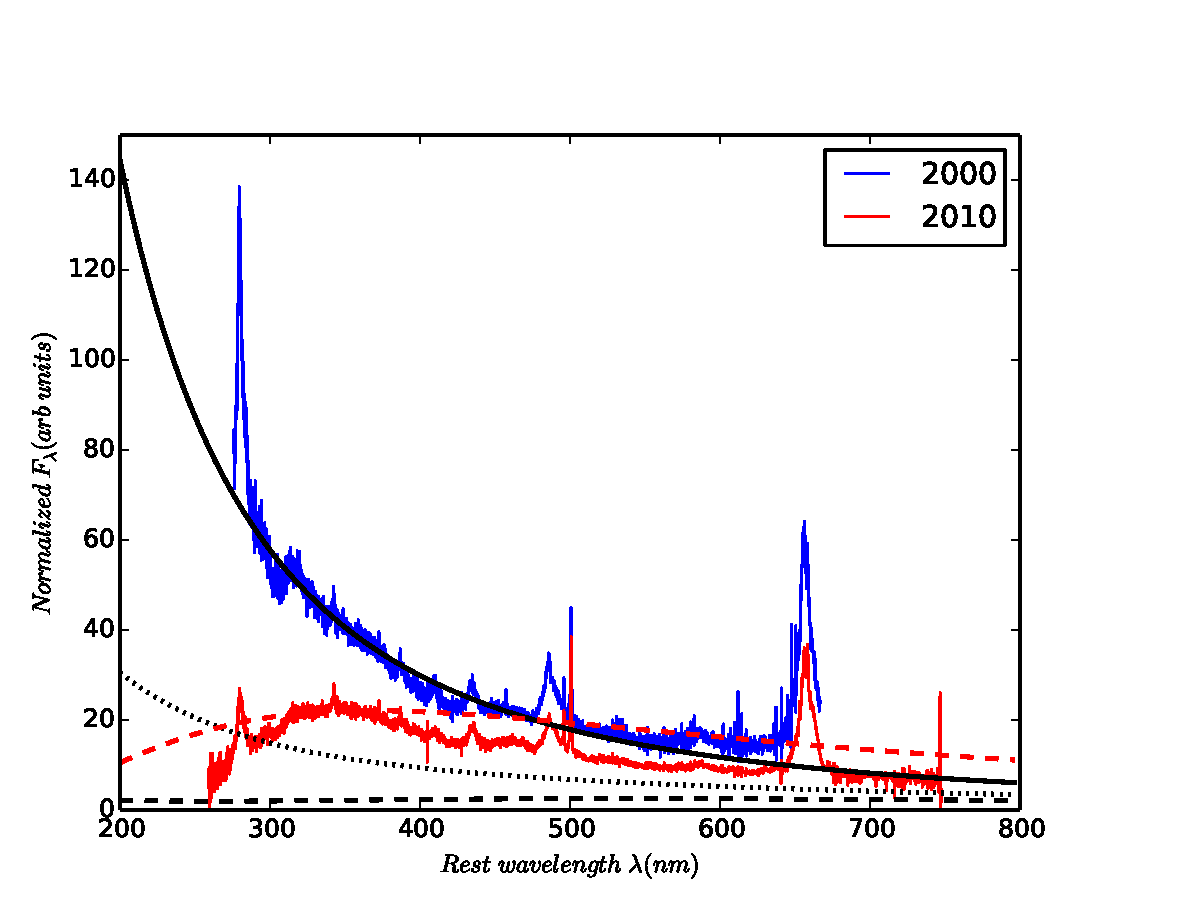
\includegraphics[width=12.00cm, height=10.0cm, trim=0.3cm 0.0cm 2.0cm 0.0cm, clip]
  {../plots/models/mcd_gap_v3_3_b1.pdf}
  \caption[]{
J1100-0053 data (blue line 2000 spectrum; red line 2010 spectrum) and 4
models. Solid black line shows non-zero torque at ISCO
\citep[following] []{Afshordi_Paczynski2003}; dotted and dashed black
lines show temperature suppression inside $r_{\rm alt} = 225 r_{\rm
g}$, such that the spectral flux is $f_{\rm dep} = $ 0.2 or 0.01
(respectively) compared to a zero torque model; dashed red line shows
zero flux inside $r_{\rm alt} = 80 r_{\rm g}$ and arbitrary
normalization to match peak of 2010 spectrum. Note the poor fit due to
the intrinsic width of the thermal peak.
  }
  \label{fig:disk_suppression}
\end{figure*}
Can J1100-0053 switch states from a thin disk quasar to an ADAF at small
radii with the thin disk surviving at large radii?  Assuming the
transition happens due to an instability on the thermal timescale of
the disk, then at large radii the thermal timescale is
\begin{equation}
    t_{\rm th} \sim 14 \; {\rm years} \; \left(\frac{\alpha}{0.03}\right)^{-1}
                                                \left(\frac{r}{225r_{g}}\right)^{3/2} 
                                                        \frac{r_{g}}{c}
\end{equation} 
and is too long given the observations. However, if the viscosity
parameter $\alpha$ increases to $\alpha \approx 0.3$, as suggested by
\citet{King2007}, then the thermal timescale is $t_{\rm th} \sim 1.4$
year and the front timescale is
\begin{equation}
    t_{\rm front}  \sim  10 \; {\rm years} \left(\frac{h/r}{0.05}\right)^{-1}
                                                           \left(\frac{\alpha}{0.3}\right)^{-1}  
                                                           \left(\frac{r}{225r_{g}}\right)^{3/2}  
                                                           \frac{r_{g}}{c}
\label{eqn:t_front}
\end{equation}
which is plausible, if there exists a very viscous disk and the effect
propagates outwards on a timescale of $\leq 10$ years from the inner
disk. This would suppress the UV/X-ray emission from the RIAF (down by
a few orders of magnitude from the intensity expected from a thin disk
intensity) and explain the broadline behaviour.  ADAF spectra are flat
in $\nu L_{\nu}$ \citet{Narayan1998, Abramowicz2002, Abramowicz2013},
and convective ADAFs rise towards X-ray energies. ADAFs exist at lower
luminosity, where $\epsilon \sim 0.005$ for $L=\epsilon \dot{M}
c^{2}$, lower than the fiducial $\epsilon \sim 0.1$ for a classic thin
disk luminosity.

However, suppressing the flux from the inner disk radii ($\lesssim 225 r_{g}$)
in the low temperature thin disk model \citep{Narayan1997, Gammie1999,
Agol_Krolik2000, Afshordi_Paczynski2003, Ford2018} by a factor of
$20$ would still not describe the 2010 spectrum. To restore the thin disk
spectrum by 2016, the disk change has to propagate back inwards, most
of the way to the ISCO and therefore $t_{\rm front}$ needs to be
shorter. This requires $h/r$ to be larger in
Equation~\ref{eqn:t_front} above, by a factor of $\sim 2$.

It is unclear what physical processes would trigger the change of
state to an ADAF and then cool back down to a thin disk. In any case,
suppressing the MCD temperature profile inside a radius of $r_{alt} =
225 r_{g}$ leads to a collapse in the total flux compared to
unperturbed disk. We show some example cases in
Figure~\ref{fig:disk_suppression}. Clearly, these scenarios are
difficult to reconcile with our data.


\smallskip \smallskip
\noindent
\textbf{\textsc{Model `B': Propogation of a Cooling Front: }}
An alternative model connected to the accretion disk is that a
\emph{cooling} front propagates through the thin disk.  In order to
reproduce the steep fall at $\lambda \leq 200$nm in the 2010 spectrum,
a cool phase leads to absorption at short wavelengths.

Initially a modestly fat disk ($h/r \sim 0.2$) with a modest $\alpha$,
cools from the ISCO and propagates outward in a cooling front,
collapsing the disk. As the hot disk ($\sim 10^{5-6}$K) cools, it
fragments into cooler clumps around $\sim 10^{4}$K \citep[see e.g.,
][]{McCourt2016}.  The main coolants $>10^{4.5}$K are resonance lines
in Carbon and Oxygen and at lower temperatures, H and He from neutral
phase material \citep[see e.g., Fig. 18 in
][]{Sutherland_Dopita1993}. The ionization energies for carbon and
oxygen are 11.26 and 13.61 eV, respectively, i.e., $\sim 100$nm, and
hence at wavelengths $<100$nm the disk opacity will increase
dramatically in an edge.  However, the gas in the disk is pressure,
turbulence and Doppler broadened, so these ionization edges will
manifest around 100nm with decreasing opacity to shorter wavelengths
as
\begin{equation}
  \kappa \propto \rho T^{-1/2} \nu^{-3}
\end{equation}
for Kramers' opacities. This implies $\kappa \propto \lambda^{3}$
at increasing wavelengths up to the ionization edge around $100$nm.
These features will be blurred (by the broadening) and the ionization 
edges due to the C and O resonance lines in the cool phase of this
disk will be span $50-200$nm, depressing the flux at these energies. 
We note this closely resembles the opacity curve inferred by \citet{Guo2016} 
in J2317+0005 over relevant wavelengths.

The 2010 spectrum in this model comes from a cooler disk plus the
increased opacity at short wavelengths in the cooler phase. Heating
occurs from the outside in, explaining the 2016 spectrum and
asymmetric recovery in photometry.  Since the
optical continuum has been rising again since mid-2016, this leads to
a prediction of a rise in Hydrogen emission line flux in the next few
months. The infrared flux returns in 2021. 



\medskip
\medskip
\medskip
\section*{Acknowledgements}
NPR acknowledges support from the STFC and the Ernest Rutherford
Fellowship scheme.  KESF \& BM are supported by NSF PAARE
AST-1153335. KESF \& BM thank CalTech/JPL for support during
sabbatical.  MF acknowledges support from NSF grants AST-1518308,
AST-1749235, AST-1413600 and NASA grant 16-ADAP16-0232.  RJA was
supported by FONDECYT grant number 1151408. AMM acknowledges
support from NASA ADAP grant NNH17AE75I.

We thank David J. Schlegel for quality checks on the BOSS data, and
Chris Done for invigorating discussions at the concept and conclusion
of this work.

This publication makes use of data products from the Wide-field
Infrared Survey Explorer, which is a joint project of the University
of California, Los Angeles, and the Jet Propulsion
Laboratory/California Institute of Technology, and NEOWISE, which is a
project of the Jet Propulsion Laboratory/California Institute of
Technology. WISE and NEOWISE are funded by the National Aeronautics
and Space Administration.

This research has made use of the NASA/IPAC Extragalactic Database
(NED) which is operated by the Jet Propulsion Laboratory, California
Institute of Technology, under contract with the National Aeronautics
and Space Administration.

This research has made use of data obtained from the SuperCOSMOS
Science Archive, prepared and hosted by the Wide Field Astronomy Unit,
Institute for Astronomy, University of Edinburgh, which is funded by
the UK Science and Technology Facilities Council.

The GALEX GR6/7 Data Release hosted at
\href{http://galex.stsci.edu/GR6/}{http://galex.stsci.edu/GR6/} was
used. These data were obtained from the Mikulski Archive for Space
Telescopes (MAST). STScI is operated by the Association of
Universities for Research in Astronomy, Inc., under NASA contract
NAS5-26555. Support for MAST for non-HST data is provided by the NASA
Office of Space Science via grant NNX09AF08G and by other grants and
contracts.

Funding for SDSS-III has been provided by the Alfred P. Sloan
Foundation, the Participating Institutions, the National Science
Foundation, and the U.S. Department of Energy Office of Science. The
SDSS-III web site is
\href{http://www.sdss3.org/}{http://www.sdss3.org/}.
%%
SDSS-III is managed by the Astrophysical Research Consortium for the
Participating Institutions of the SDSS-III Collaboration including the
University of Arizona, the Brazilian Participation Group, Brookhaven
National Laboratory, Carnegie Mellon University, University of
Florida, the French Participation Group, the German Participation
Group, Harvard University, the Instituto de Astrofisica de Canarias,
the Michigan State/Notre Dame/JINA Participation Group, Johns Hopkins
University, Lawrence Berkeley National Laboratory, Max Planck
Institute for Astrophysics, Max Planck Institute for Extraterrestrial
Physics, New Mexico State University, New York University, Ohio State
University, Pennsylvania State University, University of Portsmouth,
Princeton University, the Spanish Participation Group, University of
Tokyo, University of Utah, Vanderbilt University, University of
Virginia, University of Washington, and Yale University.




\bibliographystyle{mn2e}
\bibliography{/cos_pc19a_npr/LaTeX/tester_mnras}


\end{document}